% This is samplepaper.tex, a sample chapter demonstrating the
% LLNCS macro package for Springer Computer Science proceedings;
% Version 2.21 of 2022/01/12
%
\documentclass[runningheads]{llncs}
%
\usepackage[T1]{fontenc}
% T1 fonts will be used to generate the final print and online PDFs,
% so please use T1 fonts in your manuscript whenever possible.
% Other font encondings may result in incorrect characters.
%
\usepackage{graphicx}
% Used for displaying a sample figure. If possible, figure files should
% be included in EPS format.
%
% If you use the hyperref package, please uncomment the following two lines
% to display URLs in blue roman font according to Springer's eBook style:
%\usepackage{color}
%
\usepackage{amssymb}
%
\usepackage{multicol}
\usepackage{multirow}
\usepackage{hhline}
\usepackage{array}
\newcolumntype{C}[1]{>{\centering\arraybackslash}p{#1}}
%
\usepackage[table]{xcolor}
\definecolor{Color0}{HTML}{ffffff}
\definecolor{Color1}{HTML}{ede0d4}
\definecolor{Color2}{HTML}{e6ccb2}
\definecolor{Color3}{HTML}{ddb892}
\definecolor{Color4}{HTML}{b08968}
\definecolor{Color5}{HTML}{9c6644}
\definecolor{Color6}{HTML}{7f5539}
\definecolor{Gelo}{HTML}{D3D3D3}
%
\usepackage{diagbox}
%
\usepackage{booktabs}
%
\usepackage{amsmath}
%
\usepackage{tikz}
\usetikzlibrary{arrows.meta, positioning, quotes}
%
\usepackage{arydshln}

\usepackage{algorithm}
\usepackage{algpseudocode}

%
%\renewcommand\UrlFont{\color{blue}\rmfamily}
%\urlstyle{rm}
%
\begin{document}
%
\title{DDT Representation}
%
%\titlerunning{Abbreviated paper title}
% If the paper title is too long for the running head, you can set
% an abbreviated paper title here
%
\author{
Filipe Borba\inst{1}\orcidID{0009-0002-9428-8908}
% \and Second Author\inst{2,3}\orcidID{1111-2222-3333-4444}
% \and Third Author\inst{3}\orcidID{2222--3333-4444-5555}
}
%
\authorrunning{F. Borba et al.}
% First names are abbreviated in the running head.
% If there are more than two authors, 'et al.' is used.
%
\institute{Universidade Federal de Santa Catarina, Florianópolis SC, Brazil
% \and Springer Heidelberg, Tiergartenstr. 17, 69121 Heidelberg, Germany
% \email{lncs@springer.com}\\
% \url{http://www.springer.com/gp/computer-science/lncs}
% \and ABC Institute, Rupert-Karls-University Heidelberg, Heidelberg, Germany\\
% \email{\{abc,lncs\}@uni-heidelberg.de}
}
%
\maketitle              % typeset the header of the contribution
%
\begin{abstract}
The abstract should briefly summarize the contents of the paper in
150--250 words.

\keywords{First keyword  \and Second keyword \and Another keyword.}
\end{abstract}
%
%
%
\section{Introduction}
\label{sec:introduction}

Differential cryptanalysis, introduced by Biham and Shamir [4], is one of
the most influential statistical attacks against symmetric-key primitives.
Its central insight is that the propagation of a chosen input difference
through an iterated cipher is far from uniform, and that pairs of input and
output differences that occur with high probability can be combined into
multi-round trails that distinguish the cipher from a random permutation or
recover key material. In the decades since its introduction, the technique
has been refined into a broad family of variants, including truncated,
higher-order, impossible, and boomerang differential attacks. All of them
share the same underlying object: the difference distribution table of the
cipher's nonlinear components, which records the frequency with which each
output difference is produced by each input difference.

The size of this table is also its main limitation. For an $n$-bit S-box,
the DDT is a $2^n \times 2^n$ integer matrix, and its quadratic blow-up in
$n$ rapidly exhausts memory budgets. An $8$-bit S-box already requires $64$
KiB; beyond $n = 10$, the dense matrix can no longer be materialized on
commodity machines. As cryptanalysts increasingly turn their attention to
larger S-boxes, ARX components, and word-oriented permutations, this
exponential cost forces a recurring compromise between the expressiveness of
differential analysis and the size of the primitives that can actually be
analyzed.

Compounding this storage problem is a more subtle access problem. Even when
a DDT fits in memory, most cryptanalytic tasks do not need every cell at
once: they need to extract the small subset of entries that satisfy some
structural property. Examples are pervasive in the literature, including
enumerating all impossible differentials of an S-box, listing every $(a,b)$
that achieves the differential uniformity, isolating truncated differentials
in which only a few input bits are active, identifying entries that satisfy
a linear relation imposed by the surrounding cipher, and filtering
transitions whose probability lies above a chosen threshold. In the standard
matrix view, each of these queries is solved by an ad-hoc procedure, written
anew for every analysis, and each shares the same unavoidable lower bound:
a full or partial sweep of the table.

In this paper, we argue that the right abstraction for the DDT is not a
matrix but a formal language. By recursively partitioning the table into
quadrants, every cell is identified with a unique word over a quaternary
alphabet, and the set of words that correspond to non-zero entries forms a
regular language $L(D)$. This language is recognized by a finite
automaton whose terminal states carry the differential multiplicities, and
whose structure is canonical once a quaternary analogue of multi-terminal
binary decision diagram reduction is applied. The resulting representation
exploits both the general redundancy present in every DDT, such as the
abundance of zero entries, and the specific redundancy resulting from the
algebraic and combinatorial structure of typical S-boxes.

The compactness of this representation is, however, only one half of the
contribution. The other half, and the focus of this work, is the querying
capability that the language-theoretic view unlocks. Once the DDT is
encoded as a regular language, any subset of entries definable by a regular
condition over the alphabet $\Sigma = \{\texttt{0},\texttt{1},\texttt{2},\texttt{3}\}$ becomes a regular
language in its own right, and can be intersected with $L(D)$ using
standard automata-theoretic constructions. The disparate ad-hoc scans
listed above all collapse into a single uniform recipe: write the property
as a regular expression, compile it into a query automaton, intersect with
the DDT automaton, and enumerate the resulting language. Truncated
differentials, impossible differentials, fixed-bit differentials, entries
of extremal probability, and many other targets that have historically
required specialized code are recovered as one-line queries. Importantly,
this also lifts queries from a per-cell cost to a cost proportional to the
size of the (already compressed) intersection automaton, so the dense
matrix never has to be enumerated even implicitly.

The remainder of the paper is organized as follows. Section~\ref{sec:preliminaries} recalls the
necessary background on differential cryptanalysis and binary decision
diagrams. Section~\ref{sec:automaton} describes the construction of the DDT automaton and
its reduction. Section~\ref{sec:results} reports memory measurements on a representative
collection of S-boxes. Section~\ref{sec:applications} then turns to applications, with
Section~\ref{sec:queries} developing the query framework that motivates this work.
Section~\ref{sec:conclusion} concludes and discusses directions for future research.

\section{Preliminaries}
\label{sec:preliminaries}

This section establishes the concepts and notation used throughout this work, covering the relevant properties of differential cryptanalysis, finite automata, and decision diagrams.

\subsection{Differential Cryptanalysis}

Differential cryptanalysis is a powerful statistical attack proposed for breaking iterated block ciphers. Introduced by Biham and Shamir \cite{BihamAndShamir1991}, it analyzes how the difference between two input plaintexts behaves along the steps in the encryption process, exploiting input changes that produce certain output changes with high probability. The initial attack analyzed the structure of the cipher to find high probable differential paths or characteristics throughout the encryption process up to the last round with the intention to use this information to guess the subkey. Over time, this foundational concept has been expanded into several advanced variants, including truncated, higher-order, and impossible differential cryptanalysis.

To construct these differential characteristics, also known as differential trails, an analyst must first determine the frequencies of all possible differences propagating through the cipher's individual components. Formally, we define a pair $(a, b) \in \mathbb{F}_{2}^{n} \times \mathbb{F}_{2}^{m}$ of input and output differences as a differential and represent this relationship using the derivative of a vectorial Boolean  $F : \mathbb{F}_{2} ^{n} \to \mathbb{F}_{2}^{m}$, which calculates the output difference resulting from two inputs with a difference $a$:

\begin{equation}
    \label{eq:derivative}
    D_{a}F(x) = F(x + a) + F(x).
\end{equation}

The function $F$ typically represents a specific cipher component, such as an S-box or a round function, though it can denote any step in the encryption process.  By evaluating this derivative across all possible inputs $x$ for a fixed input difference $a$, we determine the frequency of each resulting output difference $b$. Cataloging these frequencies for every possible difference pair yields a table that completely summarizes the component's differential behavior.

\begin{definition}[Difference Distribution Table]
    Let $F$ be a vectorial Boolean Function from $\mathbb{F}_{2}^{n}$ to $\mathbb{F}_{2}^{m}$. The difference distribution table of $F$ is a $2^n \times 2^m$ matrix where the entry at row $a \in \mathbb{F}_{2^n}$ and column $b \in \mathbb{F}_{2^m}$ is defined as:

    \begin{equation}
        DDT_{F}[a, b] = \big|\{x \in \mathbb{F}_{2^n} \mid D_{a}F(x) = b\}\big|.
    \end{equation}
\end{definition}

From the DDT, an analyst can observe and calculate several properties that quantify a cipher's overall security and assist in crafting attacks. Among these properties, the most prominent and widely studied metric is the differential uniformity, in Definition 
\ref{def:differential-uniformity}. This measure represents the highest frequency of occurrence for any non-trivial differential, that is, a differential where the initial input difference is strictly non-zero. In the context of a DDT, this uniformity is readily identifiable by locating the maximum value present within the table. This peak value determines the upper bound of an attacker's success probability, and so low differential uniformity is often a primary design goal for cryptographic components.

\begin{definition}[Differential Uniformity]
    \label{def:differential-uniformity}

    Let $F$ be a vectorial Boolean function from $\mathbb{F}_{2}^{n}$ to $\mathbb{F}_{2}^{m}$. The differential uniformity of $F$, denoted by $\Delta(F)$, is the maximum number of values $x \in \mathbb{F}_{2}^{n}$ such that the derivative of $F$ with respect to $a$ in $x$ equals $b$, for some fixed values $a \ne 0 \in \mathbb{F}_{2}^{n}$ and $b \in \mathbb{F}_{2}^{m}$

    \begin{equation}
        \Delta(F) = \max_{a \ne 0, b \in \mathbb{F}_{2}^{n}} \big| \{x \in \mathbb{F}_{2}^{n} : D_{a}F(x) = b\} \big|.
    \end{equation}
\end{definition}

However, differential uniformity is not the sole indicator of cryptographic security. Functions optimized exclusively for this metric often correspond to mathematical objects possessing strong algebraic structures, which can introduce alternative vulnerabilities. Such weaknesses have been exploited in various attacks, such as \cite{JakobsenAndKnudsen1997}, \cite{CourtoisAndPieprzyk2002}, and \cite{CanteautAndVideu2002}. Consequently, a cipher's resistance is affected by a broader range of differential properties. An example is the differential spectrum. While the differential uniformity isolates the single maximum frequency value, the differential spectrum provides a distribution of all entries in the table.

\begin{definition}[Differential spectrum]
    \label{def:differential-spectrum}

    Let $F$ be a vectorial Boolean function. The differential spectrum of $F$ is the multiset of values

    \begin{equation*}
        \big| \{ x \in \mathbb{F}_{2}^{n} \mid D_{a}F(x) = b \} \big|
    \end{equation*}
    over all $a \neq 0 \in \mathbb{F}_{2}^{n}$ and $b \in \mathbb{F}_{2}^{m}$. The elements in this multiset are represented by $\omega_{i}$, where each $\omega_{i}$ denotes the number of non-trivial differentials $(a, b)$ that occur $i$ times in $F$.
\end{definition}

Additionally, the table reveals other features of the component represented, such as impossible differentials, which are pairs of input and output differences that never occur, corresponding to the zero entries in the table. To efficiently analyze these specific paths, analysts often use a *-DDT. Unlike a conventional DDT that records the exact frequency of every differential, a *-DDT acts as a boolean matrix that indicates only whether a transition is possible or impossible. From an attacker's perspective, these impossible transitions serve as a powerful filtering mechanism. In an impossible differential attack, the cryptanalyst guesses parts of the key and partially decrypts the ciphertexts; if a guessed subkey leads to a difference transition that is known to be impossible, that subkey is proven incorrect and discarded.

\subsection{Binary Decision Diagrams}

The efficient representation of Boolean functions is a fundamental problem. Because truth tables grow exponentially with the number of variables, graph-based data structures known as binary decision diagrams, or BDDs, were developed to offer a more compact alternative. While initial concepts were proposed by Lee \cite{Lee1959} and Akers \cite{Akers1978}, it was Bryant who introduced strict variable ordering and reduction rules, establishing BDDs as a practical and canonical representation.

\begin{definition}[Binary Decision Diagram]
\label{def:state-equivalence}
    A Binary Decision Diagram is a rooted, directed acyclic graph with a vertex set $V$ partitioned into non-terminal and terminal vertices. Each non-terminal vertex $v \in V$ is has an attribute $\operatorname{index}(v)$ in $\mathbb{N}$ and has two child vertices, denoted as $\operatorname{low}(v)$ and $\operatorname{high}(v)$. Each terminal vertex $u \in V$ is labeled by a Boolean value $\operatorname{value}(u) \in \{0, 1\}$.
\end{definition}

Evaluating a Boolean function with a BDD involves traversing the graph from the root to a terminal vertex. Given a decision diagram representing a function $f(x_{1}, x_{2}, \dots, x_{n})$, the traversal begins at the root and, at each non-terminal vertex $v$ with $\operatorname{index}(v) = i$, the path advances to $\operatorname{low}(v)$ if its associated variable $x_{i}$ is $0$, and to $\operatorname{high}(v)$ otherwise. This process continues until a terminal node $u$ is reached, at which point the BDD yields $\operatorname{value}(u)$ as the final output of the function.

Although a standard BDD provides a valid model for Boolean functions, it is neither canonical nor minimal. The exact structure of the graph is highly dependent on the evaluation order, meaning the same function can yield different representations. To resolve these inefficiencies, Bryant \cite{Bryant1986} introduced reduced ordered binary decision diagrams, or ROBDDs. This data structure provides a compact, canonical form that enables efficient algorithmic manipulation by imposing a strict variable ordering alongside reduction rules.

\begin{definition}[Reduced Ordered Binary Decision Diagram]
A BDD is ordered if there exists a strict total ordering over the set of variables such that for every non-terminal vertex $v$, the variables of its non-terminal children $\operatorname{low}(v)$ and $\operatorname{high}(v)$ strictly follow $\operatorname{index}(v)$ in the ordering. It is reduced if it satisfies two conditions: (1) it contains no vertex $v$ where $\operatorname{low}(v) = \operatorname{high}(v)$, and (2) it contains no distinct vertices $u$ and $v$ such that the subgraphs rooted at these vertices are isomorphic.
\end{definition}

The strict variable ordering combined with the reduction rules transforms the BDD into a canonical and minimal representation. This canonical property guarantees that equivalent Boolean functions will map to the exact same graph. Moreover, minimality allows complex data to be represented with significant storage efficiency.

A limitation of the previous representations is the restriction of terminal nodes to {0, 1}. While suitable for Boolean logic, representing general integer-valued matrices requires a broader range of values. A multi-terminal binary decision diagram, or MTBDD, proposed by Fujita et al. \cite{FujitaEtAl1997}, addresses this by allowing terminal nodes to take arbitrary values from a finite set. By encoding matrix indices as Boolean variables, an MTBDD represents an entire integer-valued matrix. Retaining the strict variable ordering and reduction rules of an ROBDD yields a compressed, canonical representation.

\begin{definition}
    A multi-terminal binary decision diagram is a rooted, directed acyclic graph representing a function $f: \{0, 1\}^n \to S$, where $S$ is an arbitrary finite set. It extends the conventional binary decision diagram by allowing terminal nodes to take values from $S$ instead of being restricted to $\{0, 1\}$.
\end{definition}
\section{An Automaton-Theoretic Representation of DDTs}
\label{sec:automaton}

The presents a novel DDT representation using automaton theory based on the hypothesis that the derivative of functions used as S-boxes in popular ciphers are not random, but possess significant structural regularities that can be exploited for compression. We first point the fundamental limitations of representing the DDT as a dense matrix and then introduce a representation, showing the process to convert a DDT into an automaton using less storage.

\subsection{Structural Redundancy in DDTs}
\label{sec:redundancies}

For an $n$-bit S-box, the representation of its DDT as a matrix requires $2^{2n}$ elements, which quickly becomes prohibitive for storage, and in-memory analysis as $n$ increases. The inefficiency of this representation is the result of two types of redundancy. The first is the general redundancy present in every DDT: because the number of distinct differential values is significantly smaller than the total number of cells, many cells have the same value. For instance, at least half of the DDT entries are always zero. The second is the specific redundancy resulting from the properties of the S-box, which manifests as the frequent repetition of small, identical patterns or blocks throughout the table.

This specific redundancy is particularly visible in the DDT of the PRESENT S-box, as illustrated in Table~\ref{tab:present_ddt_blocks}. In this visualization, the table is partitioned into $2 \times 2$ blocks, and colors are assigned to each according to its frequency: higher frequency of blocks receive darker colors while less frequent blocks receive lighter ones. In this particular case, 25 out of 64 blocks in the table falls into only 3 block patterns, with the all-zero block having 11 occurrences. This provides a hint that we can use the same structure to represent a significant portion of the DDT.

\begin{table}
    \caption{The DDT of the PRESENT S-box, partitioned into 2×2 blocks. Blocks with the same frequency share the same color.}
    \label{tab:present_ddt_blocks}
    
    \centering

    \begin{tabular}{|*{8}{w{c}{0.03\textwidth}w{c}{0.03\textwidth}|}}

        \hline
        
        \cellcolor{Color6}\textcolor{Gelo}0 &
        \cellcolor{Color6}\textcolor{Gelo}0 &
        \cellcolor{Color4}0 & \cellcolor{Color4}0 & 
        \cellcolor{Color6}\textcolor{Gelo}0 & \cellcolor{Color6}\textcolor{Gelo}0 & 
        \cellcolor{Color4}0 & \cellcolor{Color4}0 &
        \cellcolor{Color4}0 & \cellcolor{Color4}0 & 
        \cellcolor{Color6}\textcolor{Gelo}0 & \cellcolor{Color6}\textcolor{Gelo}0 &
        \cellcolor{Color4}0 & \cellcolor{Color4}0 & \cellcolor{Color6}\textcolor{Gelo}0 & \cellcolor{Color6}\textcolor{Gelo}0 \\
        
        \cellcolor{Color6}\textcolor{Gelo}0 & \cellcolor{Color6}\textcolor{Gelo}0 &
        \cellcolor{Color4}0 & \cellcolor{Color4}4 & \cellcolor{Color6}\textcolor{Gelo}0 & \cellcolor{Color6}\textcolor{Gelo}0 &
        \cellcolor{Color4}0 & \cellcolor{Color4}4 &
        \cellcolor{Color4}0 & \cellcolor{Color4}4 & \cellcolor{Color6}\textcolor{Gelo}0 & \cellcolor{Color6}\textcolor{Gelo}0 &
        \cellcolor{Color4}0 & \cellcolor{Color4}4 & \cellcolor{Color6}\textcolor{Gelo}0 & \cellcolor{Color6}\textcolor{Gelo}0 \\
        
        \hline
        
        \cellcolor{Color3}0 & \cellcolor{Color3}0 & \cellcolor{Color3}0 & \cellcolor{Color3}2 & \cellcolor{Color3}0 & \cellcolor{Color3}4 & \cellcolor{Color3}2 & \cellcolor{Color3}0 & \cellcolor{Color6}\textcolor{Gelo}0 & \cellcolor{Color6}\textcolor{Gelo}0 &
        \cellcolor{Color3}2 & \cellcolor{Color3}0 & \cellcolor{Color5}2 & \cellcolor{Color5}2 &
        \cellcolor{Color3}2 & \cellcolor{Color3}0 \\
        
        \cellcolor{Color3}0 & \cellcolor{Color3}2 & \cellcolor{Color3}0 & \cellcolor{Color3}2 & \cellcolor{Color3}2 & \cellcolor{Color3}0 & \cellcolor{Color3}4 & \cellcolor{Color3}2 & \cellcolor{Color6}\textcolor{Gelo}0 & \cellcolor{Color6}\textcolor{Gelo}0 &
        \cellcolor{Color3}2 & \cellcolor{Color3}2 & \cellcolor{Color5}0 & \cellcolor{Color5}0 &
        \cellcolor{Color3}0 & \cellcolor{Color3}0 \\
        
        \hline
        
        \cellcolor{Color3}0 & \cellcolor{Color3}0 & \cellcolor{Color6}\textcolor{Gelo}0 & \cellcolor{Color6}\textcolor{Gelo}0 &
        \cellcolor{Color3}0 & \cellcolor{Color3}4 & \cellcolor{Color5}2 & \cellcolor{Color5}2 &
        \cellcolor{Color3}0 & \cellcolor{Color3}2 & \cellcolor{Color3}2 & \cellcolor{Color3}0 & \cellcolor{Color3}2 & \cellcolor{Color3}0 & \cellcolor{Color3}2 & \cellcolor{Color3}0 \\
        
        \cellcolor{Color3}0 & \cellcolor{Color3}2 & \cellcolor{Color6}\textcolor{Gelo}0 & \cellcolor{Color6}\textcolor{Gelo}0 &
        \cellcolor{Color3}2 & \cellcolor{Color3}0 & \cellcolor{Color5}0 & \cellcolor{Color5}0 &
        \cellcolor{Color3}0 & \cellcolor{Color3}2 & \cellcolor{Color3}2 & \cellcolor{Color3}2 & \cellcolor{Color3}4 & \cellcolor{Color3}2 & \cellcolor{Color3}0 & \cellcolor{Color3}0 \\ 
        
        \hline
        
        \cellcolor{Color4}0 & \cellcolor{Color4}0 &
        \cellcolor{Color3}2 & \cellcolor{Color3}0 & \cellcolor{Color6}\textcolor{Gelo}0 & \cellcolor{Color6}\textcolor{Gelo}0 &
        \cellcolor{Color3}2 & \cellcolor{Color3}0 & \cellcolor{Color3}2 & \cellcolor{Color3}0 & \cellcolor{Color2}0 & \cellcolor{Color2}4 & \cellcolor{Color3}2 & \cellcolor{Color3}0 &
        \cellcolor{Color1}0 & \cellcolor{Color1}4 \\
        
        \cellcolor{Color4}0 & \cellcolor{Color4}4 &
        \cellcolor{Color3}2 & \cellcolor{Color3}0 & \cellcolor{Color6}\textcolor{Gelo}0 & \cellcolor{Color6}\textcolor{Gelo}0 &
        \cellcolor{Color3}2 & \cellcolor{Color3}0 & \cellcolor{Color3}2 & \cellcolor{Color3}0 & \cellcolor{Color2}0 & \cellcolor{Color2}0 & \cellcolor{Color3}2 & \cellcolor{Color3}0 &
        \cellcolor{Color1}0 & \cellcolor{Color1}4 \\
        
        \hline
        
        \cellcolor{Color6}\textcolor{Gelo}0 & \cellcolor{Color6}\textcolor{Gelo}0 &
        \cellcolor{Color3}0 & \cellcolor{Color3}2 & \cellcolor{Color2}0 & \cellcolor{Color2}0 & \cellcolor{Color3}0 & \cellcolor{Color3}2 & \cellcolor{Color3}0 & \cellcolor{Color3}2 & \cellcolor{Color2}0 & \cellcolor{Color2}4 & \cellcolor{Color3}0 & \cellcolor{Color3}2 &
        \cellcolor{Color1}0 & \cellcolor{Color1}4 \\
        
        \cellcolor{Color6}\textcolor{Gelo}0 & \cellcolor{Color6}\textcolor{Gelo}0 &
        \cellcolor{Color3}2 & \cellcolor{Color3}0 & \cellcolor{Color2}4 & \cellcolor{Color2}0 & \cellcolor{Color3}2 & \cellcolor{Color3}0 & \cellcolor{Color3}2 & \cellcolor{Color3}0 & \cellcolor{Color2}0 & \cellcolor{Color2}0 & \cellcolor{Color3}2 & \cellcolor{Color3}0 &
        \cellcolor{Color1}4 & \cellcolor{Color1}0 \\
        
        \hline
        
        \cellcolor{Color3}0 & \cellcolor{Color3}0 & \cellcolor{Color5}2 & \cellcolor{Color5}2 &
        \cellcolor{Color3}0 & \cellcolor{Color3}4 & \cellcolor{Color6}\textcolor{Gelo}0 & \cellcolor{Color6}\textcolor{Gelo}0 &
        \cellcolor{Color3}2 & \cellcolor{Color3}0 & \cellcolor{Color3}2 & \cellcolor{Color3}0 & \cellcolor{Color3}0 & \cellcolor{Color3}2 & \cellcolor{Color3}2 & \cellcolor{Color3}0 \\
        
        \cellcolor{Color3}0 & \cellcolor{Color3}2 & \cellcolor{Color5}0 & \cellcolor{Color5}0 &
        \cellcolor{Color3}2 & \cellcolor{Color3}0 & \cellcolor{Color6}\textcolor{Gelo}0 & \cellcolor{Color6}\textcolor{Gelo}0 &
        \cellcolor{Color3}4 & \cellcolor{Color3}2 & \cellcolor{Color3}2 & \cellcolor{Color3}2 & \cellcolor{Color3}0 & \cellcolor{Color3}2 & \cellcolor{Color3}0 & \cellcolor{Color3}0 \\
        
        \hline
        
        \cellcolor{Color3}0 & \cellcolor{Color3}0 & \cellcolor{Color3}2 & \cellcolor{Color3}0 & \cellcolor{Color3}0 & \cellcolor{Color3}4 & \cellcolor{Color3}0 & \cellcolor{Color3}2 & \cellcolor{Color5}2 & \cellcolor{Color5}2 &
        \cellcolor{Color3}2 & \cellcolor{Color3}0 & \cellcolor{Color6}\textcolor{Gelo}0 & \cellcolor{Color6}\textcolor{Gelo}0 &
        \cellcolor{Color3}2 & \cellcolor{Color3}0 \\
        
        \cellcolor{Color3}0 & \cellcolor{Color3}2 & \cellcolor{Color3}4 & \cellcolor{Color3}2 & \cellcolor{Color3}2 & \cellcolor{Color3}0 & \cellcolor{Color3}0 & \cellcolor{Color3}2 & \cellcolor{Color5}0 & \cellcolor{Color5}0 &
        \cellcolor{Color3}2 & \cellcolor{Color3}2 & \cellcolor{Color6}\textcolor{Gelo}0 & \cellcolor{Color6}\textcolor{Gelo}0 &
        \cellcolor{Color3}0 & \cellcolor{Color3}0 \\
        
        \hline
        
        \cellcolor{Color4}0 & \cellcolor{Color4}0 & \cellcolor{Color5}2 & \cellcolor{Color5}2 &
        \cellcolor{Color2}0 & \cellcolor{Color2}0 & \cellcolor{Color5}2 & \cellcolor{Color5}2 &
        \cellcolor{Color5}2 & \cellcolor{Color5}2 &
        \cellcolor{Color6}\textcolor{Gelo}0 & \cellcolor{Color6}\textcolor{Gelo}0 &
        \cellcolor{Color5}2 & \cellcolor{Color5}2 &
        \cellcolor{Color1}0 & \cellcolor{Color1}0 \\
         
        \cellcolor{Color4}0 & \cellcolor{Color4}4 & \cellcolor{Color5}0 & \cellcolor{Color5}0 &
        \cellcolor{Color2}4 & \cellcolor{Color2}0 & \cellcolor{Color5}0 & \cellcolor{Color5}0 &
        \cellcolor{Color5}0 & \cellcolor{Color5}0 &
        \cellcolor{Color6}\textcolor{Gelo}0 & \cellcolor{Color6}\textcolor{Gelo}0 &
        \cellcolor{Color5}0 & \cellcolor{Color5}0 &
        \cellcolor{Color1}4 & \cellcolor{Color1}4 \\
        
        \hline
    
    \end{tabular}

    \vspace{0.25em}

    \begin{center}
    \footnotesize
    \textbf{Legend} \par

    \begin{tabular}{*{3}{w{c}{0.03\textwidth}rl}}
         \\

         \cellcolor{Color6} & \ 11 & occurrences \ &
         \cellcolor{Color5}\phantom{XX} & \ 8 & occurrences \ &
         \cellcolor{Color4}\phantom{XX} & \ 6 & occurrences \\
         \cellcolor{Color3}\phantom{XX} & \ 4 & occurrences \ &
         \cellcolor{Color2}\phantom{XX} & \ 2 & occurrences \ &
         \cellcolor{Color1}\phantom{XX} & \ 1 & occurrence \\
    \end{tabular}
    \end{center}
\end{table}


To capture both general and specific regularities of DDTs, we propose a method that reframes these tables as formal languages and represents them using finite automata. This approach draws from techniques used in image compression and Boolean functions representation and provides a canonical and compressed representation of a DDT.

\subsection{Constructing a finite automaton from a DDT}

To transform a DDT into a finite automaton, we employ techniques established in \cite{BerstelAndMorcrette} and \cite{BerstelAndNaitAbdallah}. Let $\Sigma = \{0, 1, 2, 3\}$ be a quaternary alphabet. We assign the whole matrix the empty string $\varepsilon$. Then, we partition the $2^{n} \times 2^{n}$ DDT matrix into four equal $2^{n - 1} \times 2^{n - 1}$ quadrants, assigning a distinct symbol from $\Sigma$ to each. This partitioning is applied recursively, subdividing each subsequent sub-matrix. If a sub-matrix is assigned the string $w$, its four quadrants are assigned strings $wa$ for each $a$ in $\Sigma$. This process continues until reaching the individual cells that represent the differential uniformity values. Consequently, the coordinates of each cell in the DDT are mapped to a set of strings S. The subset of $S$ comprising strings that correspond to non-zero entries of the DDT we call the language of the DDT, and denote by $L(DDT)$. Figure~\ref{fig:encoding_example} illustrates this recursive assigning scheme in detail for an $8 \times 8$ DDT. In (a), the initial DDT is first partitioned into four primary quadrants, each represented by a single symbol from $\Sigma$. This recursive subdivision is demonstrated further in (b), where each sub-quadrant is assigned a string of length two by appending symbols to the string of its containing quadrant. This partitioning reaches the individual cell level in (c), where the highlighted cell is uniquely encoded by the string \texttt{320}."

\begin{figure}
    \caption{Recursive quadrant encoding of an $8 \times 8$ DDT. Item (a) shows the whole table divided into 4 quadrants; Item (b) shows each quadrant further divided into 4 subquadrants; Item (c) highlights the cell encoded as \texttt{320}.}
    \label{fig:encoding_example}

    \centering

    \vspace{1em}

    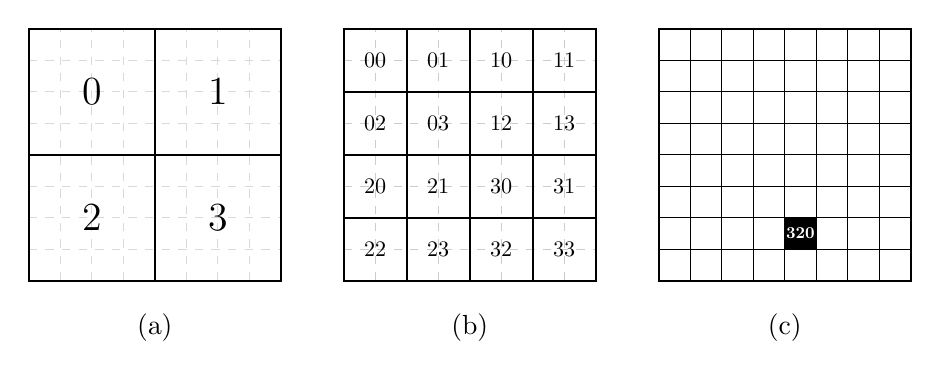
\begin{tikzpicture}[scale=0.4]
        \begin{scope}[shift={(0,0)}]
            \draw[step=1, gray!30, thin, dashed] (0,0) grid (8,8);
            \draw[thick] (0,0) rectangle (8,8);
            \draw[thick] (4,0) -- (4,8);
            \draw[thick] (0,4) -- (8,4);
            
            \node at (2,6) {\Large 0};
            \node at (6,6) {\Large 1};
            \node at (2,2) {\Large 2};
            \node at (6,2) {\Large 3};
            \node at (4,-1.5) {\normalsize (a)};
        \end{scope}

        \begin{scope}[shift={(10,0)}]
            \draw[step=1, gray!40, thin, dashed] (0,0) grid (8,8);
            \draw[thick] (0,0) rectangle (8,8);
            \draw[thick] (4,0) -- (4,8);
            \draw[thick] (0,4) -- (8,4);
            \draw[thick] (2,0) -- (2,8); \draw[thick] (6,0) -- (6,8);
            \draw[thick] (0,2) -- (8,2); \draw[thick] (0,6) -- (8,6);

            \foreach \x/\y/\label in {1/7/00, 3/7/01, 1/5/02, 3/5/03, 5/7/10, 7/7/11, 5/5/12, 7/5/13, 1/3/20, 3/3/21, 1/1/22, 3/1/23, 5/3/30, 7/3/31, 5/1/32, 7/1/33} {
                \node[scale=0.8] at (\x,\y) {\normalsize \label};
            }
            \node at (4,-1.5) {\normalsize (b)};
        \end{scope}

        \begin{scope}[shift={(20,0)}]
            \draw[step=1, thin] (0,0) grid (8,8);
            \draw[thick] (0,0) rectangle (8,8);
            
            \fill[black] (4,1) rectangle (5,2); 
            \node[scale=0.6, text=white, font=\bfseries] at (4.5,1.5) {320};
            \node at (4,-1.5) {\normalsize (c)};
        \end{scope}
    \end{tikzpicture}
\end{figure}






% \begin{table}[ht]
%     \caption{Recursive quadrant encoding representations.}
%     \label{tab:encoding_example}
%     \centering
%     \renewcommand{\arraystretch}{1.0}
%     \setlength{\tabcolsep}{4pt}
%     \begin{tabular}{c@{\hskip 0.3in}c@{\hskip 0.3in}c}
%         \begin{tabular}{|*{8}{c|}}
%         \hline
%         ~ & ~ & ~ & ~ & ~ & ~ & ~ & ~ \\ \hline
%         ~ & ~ & ~ & ~ & ~ & ~ & ~ & ~ \\ \hline
%         ~ & ~ & ~ & ~ & ~ & ~ & ~ & ~ \\ \hline
%         ~ & ~ & ~ & ~ & ~ & ~ & ~ & ~ \\ \hline
%         ~ & ~ & ~ & ~ & ~ & ~ & ~ & ~ \\ \hline
%         ~ & ~ & ~ & ~ & ~ & ~ & ~ & ~ \\ \hline
%         ~ & ~ & ~ & ~ & ~ & ~ & ~ & ~ \\ \hline
%         ~ & ~ & ~ & ~ & ~ & ~ & ~ & ~ \\ \hline
%         \end{tabular}
%         &
%         \begin{tabular}{|*{8}{c|}}
%         \hline
%         ~ & ~ & ~ & ~ & ~ & ~ & ~ & ~ \\ \hline
%         ~ & ~ & ~ & ~ & ~ & ~ & ~ & ~ \\ \hline
%         ~ & ~ & ~ & ~ & ~ & ~ & ~ & ~ \\ \hline
%         ~ & ~ & ~ & ~ & ~ & ~ & ~ & ~ \\ \hline
%         ~ & ~ & ~ & ~ & ~ & ~ & ~ & ~ \\ \hline
%         ~ & ~ & ~ & ~ & ~ & ~ & ~ & ~ \\ \hline
%         ~ & ~ & ~ & ~ & ~ & ~ & ~ & ~ \\ \hline
%         ~ & ~ & ~ & ~ & ~ & ~ & ~ & ~ \\ \hline
%         \end{tabular}
%         &
%         \begin{tabular}{|*{8}{c|}}
%         \hline
%         ~ & ~ & ~ & ~ & ~ & ~ & ~ & ~ \\ \hline
%         ~ & ~ & ~ & ~ & ~ & ~ & ~ & ~ \\ \hline
%         ~ & ~ & ~ & ~ & ~ & ~ & ~ & ~ \\ \hline
%         ~ & ~ & ~ & ~ & ~ & ~ & ~ & ~ \\ \hline
%         ~ & ~ & ~ & ~ & ~ & ~ & ~ & ~ \\ \hline
%         ~ & ~ & ~ & ~ & ~ & ~ & ~ & ~ \\ \hline
%         ~ & ~ & ~ & ~ & ~ & ~ & ~ & ~ \\ \hline
%         ~ & ~ & ~ & ~ & ~ & ~ & ~ & ~ \\ \hline
%         \end{tabular} \\
%         (a) & (b) & (c)
%     \end{tabular}
% \end{table}



% \begin{table}
%     \caption{Recursive quadrant encoding for a $8 \times 8$ DDT. Each cell is uniquely identified by a 4-symbol word. For example, the highlighted region corresponds to all words with the prefix \texttt{320}.}
%     \label{tab:encoding_example}
    
%     \centering
%     \renewcommand{\arraystretch}{1.4}
%     \ttfamily
    
%     \begin{tabular}{|*{16}{C{0.08\textwidth}|}}
    
%     \hline

%     \multicolumn{8}{|C{0.32\textwidth}|}{\multirow{8}{*}{\Huge 0}} & \multicolumn{4}{C{0.16\textwidth}|}{\multirow{4}{*}{\Large 10}} & \multicolumn{4}{C{0.16\textwidth}|}{\multirow{4}{*}{\Large 11}} \\
%     \multicolumn{8}{|C{0.08\textwidth}|}{}                         & \multicolumn{4}{C{0.08\textwidth}|}{}                           & \multicolumn{4}{C{0.08\textwidth}|}{}                           \\
%     \multicolumn{8}{|C{0.08\textwidth}|}{}                         & \multicolumn{4}{C{0.08\textwidth}|}{}                           & \multicolumn{4}{C{0.08\textwidth}|}{}                           \\
%     \multicolumn{8}{|C{0.08\textwidth}|}{}                         & \multicolumn{4}{C{0.08\textwidth}|}{}                           & \multicolumn{4}{C{0.08\textwidth}|}{}                           \\
    
%     \cline{9-16}
    
%     \multicolumn{8}{|C{0.08\textwidth}|}{}                         & \multicolumn{4}{C{0.16\textwidth}|}{\multirow{4}{*}{\Large 12}} & \multicolumn{4}{C{0.16\textwidth}|}{\multirow{4}{*}{\Large 13}} \\
%     \multicolumn{8}{|C{0.08\textwidth}|}{}                         & \multicolumn{4}{C{0.08\textwidth}|}{}                           & \multicolumn{4}{C{0.08\textwidth}|}{}                           \\
%     \multicolumn{8}{|C{0.08\textwidth}|}{}                         & \multicolumn{4}{C{0.08\textwidth}|}{}                           & \multicolumn{4}{C{0.08\textwidth}|}{}                           \\
%     \multicolumn{8}{|C{0.08\textwidth}|}{}                         & \multicolumn{4}{C{0.08\textwidth}|}{}                           & \multicolumn{4}{C{0.08\textwidth}|}{}                           \\
    
%     \hline
    
%     \multicolumn{2}{|C{0.08\textwidth}|}{\multirow{2}{*}{200}} & \multicolumn{2}{C{0.08\textwidth}|}{\multirow{2}{*}{201}} & \multicolumn{2}{C{0.08\textwidth}|}{\multirow{2}{*}{210}} & \multicolumn{2}{C{0.08\textwidth}|}{\multirow{2}{*}{211}} & \multicolumn{2}{C{0.08\textwidth}|}{\multirow{2}{*}{300}}  & \multicolumn{2}{C{0.08\textwidth}|}{\multirow{2}{*}{301}} & \multicolumn{2}{C{0.08\textwidth}|}{\multirow{2}{*}{310}} & \multicolumn{2}{C{0.08\textwidth}|}{\multirow{2}{*}{311}} \\
    
%     \multicolumn{2}{|C{0.08\textwidth}|}{}                     & \multicolumn{2}{C{0.08\textwidth}|}{}                     & \multicolumn{2}{C{0.08\textwidth}|}{}                     & \multicolumn{2}{C{0.08\textwidth}|}{}                     & \multicolumn{2}{C{0.08\textwidth}|}{}                      & \multicolumn{2}{C{0.08\textwidth}|}{}                     & \multicolumn{2}{C{0.08\textwidth}|}{}                         & \multicolumn{2}{C{0.08\textwidth}|}{}                     \\ 
    
%     \cline{1-16}
    
%     % Row 11-12: Sub-quadrants 20 and 21 (left), 30 and 31 (right)
%     \multicolumn{2}{|C{0.08\textwidth}|}{\multirow{2}{*}{202}} & \multicolumn{2}{C{0.08\textwidth}|}{\multirow{2}{*}{203}} & \multicolumn{2}{C{0.08\textwidth}|}{\multirow{2}{*}{212}} & \multicolumn{2}{C{0.08\textwidth}|}{\multirow{2}{*}{213}} & \multicolumn{2}{C{0.08\textwidth}|}{\multirow{2}{*}{302}}  & \multicolumn{2}{C{0.08\textwidth}|}{\multirow{2}{*}{303}} & \multicolumn{2}{C{0.08\textwidth}|}{\multirow{2}{*}{312}} & \multicolumn{2}{C{0.08\textwidth}|}{\multirow{2}{*}{313}} \\
    
%     \multicolumn{2}{|C{0.08\textwidth}|}{}                     & \multicolumn{2}{C{0.08\textwidth}|}{}                     & \multicolumn{2}{C{0.08\textwidth}|}{}                     & \multicolumn{2}{C{0.08\textwidth}|}{}                     & \multicolumn{2}{C{0.08\textwidth}|}{}                      & \multicolumn{2}{C{0.08\textwidth}|}{}                     & \multicolumn{2}{C{0.08\textwidth}|}{}                         & \multicolumn{2}{C{0.08\textwidth}|}{}                     \\
    
%     \hline
    
%     % Row 13-14: Sub-quadrants 22 and 23 (left), 32 and 33 (right)
%     \multicolumn{2}{|C{0.08\textwidth}|}{\multirow{2}{*}{220}}  & \multicolumn{2}{C{0.08\textwidth}|}{\multirow{2}{*}{221}} & \multicolumn{2}{C{0.08\textwidth}|}{\multirow{2}{*}{230}} & \multicolumn{2}{C{0.08\textwidth}|}{\multirow{2}{*}{231}} & \multicolumn{2}{C{0.08\textwidth}|}{\cellcolor{Color1}\multirow{2}{*}{320}} & \multicolumn{2}{C{0.08\textwidth}|}{\multirow{2}{*}{321}} & \multicolumn{2}{C{0.08\textwidth}|}{\multirow{2}{*}{330}} & \multicolumn{2}{C{0.08\textwidth}|}{\multirow{2}{*}{331}} \\
    
%     \multicolumn{2}{|C{0.08\textwidth}|}{}                      & \multicolumn{2}{C{0.08\textwidth}|}{}                     & \multicolumn{2}{C{0.08\textwidth}|}{}                     & \multicolumn{2}{C{0.08\textwidth}|}{}                     & \multicolumn{2}{C{0.08\textwidth}|}{\cellcolor{Color1}\multirow{-2}{*}{320}}                     & \multicolumn{2}{C{0.08\textwidth}|}{}                     & \multicolumn{2}{C{0.08\textwidth}|}{}                     & \multicolumn{2}{C{0.08\textwidth}|}{}                     \\
    
%     \cline{1-16}
    
%     % Row 15-16: Sub-quadrants 22 and 23 (left), 32 and 33 (right)
%     \multicolumn{2}{|C{0.08\textwidth}|}{\multirow{2}{*}{222}} & \multicolumn{2}{C{0.08\textwidth}|}{\multirow{2}{*}{223}} & \multicolumn{2}{C{0.08\textwidth}|}{\multirow{2}{*}{232}} & \multicolumn{2}{C{0.08\textwidth}|}{\multirow{2}{*}{233}} & \multicolumn{2}{C{0.08\textwidth}|}{\multirow{2}{*}{322}} & \multicolumn{2}{C{0.08\textwidth}|}{\multirow{2}{*}{323}} & \multicolumn{2}{C{0.08\textwidth}|}{\multirow{2}{*}{332}} & \multicolumn{2}{C{0.08\textwidth}|}{\multirow{2}{*}{333}} \\
    
%     \multicolumn{2}{|C{0.08\textwidth}|}{}                     & \multicolumn{2}{C{0.08\textwidth}|}{}                     & \multicolumn{2}{C{0.08\textwidth}|}{}                     & \multicolumn{2}{C{0.08\textwidth}|}{}                     & \multicolumn{2}{C{0.08\textwidth}|}{}                     & \multicolumn{2}{C{0.08\textwidth}|}{}                     & \multicolumn{2}{C{0.08\textwidth}|}{}                          & \multicolumn{2}{C{0.08\textwidth}|}{}                     \\
    
%     \hline
    
%     \end{tabular}
% \end{table}


Following the structural mapping, $L(DDT)$ is represented by a quaternary finite automaton where each path from the initial state to a terminal state corresponds to a word $w \in \Sigma^{n}$. In this construction, the internal states represent the sub-matrices generated during the recursive partition, while the transitions are dictated by the symbols of the alphabet $\Sigma$. Unlike standard finite automata, which only outputs 0 or 1 to either accept or reject, this automaton must output the values in the DDT. To achieve this, we define a function $f_{D} : \Sigma^{n} \to \mathbb{N}$. Consequently, the evaluation of any word $w \in \Sigma^{n}$ not only verifies if the corresponding differential is possible but also returns its number of occurrences.

To optimize storage, minimization is necessary. But since standard automata evaluate to 0 or 1 only, classical minimization algorithms cannot be directly applied; otherwise, they would merge accept states that refer to different values in the DDT. Specifically, we draw upon the relationship between finite automata and decision diagrams \cite{KimuraAndClarke1990} and multi-terminal binary decision diagrams, which extend standard binary decision diagrams by allowing arbitrary integer terminals \cite{FujitaEtAl1997}. By combining these concepts, we create a quaternary variant of a multi-terminal decision diagram to represent and minimize our automaton.

The compression process corresponds directly to the reductions of this decision diagram, which is achieved by eliminating redundant vertices and duplicate subgraphs. Because our alphabet contains four symbols, we modify traditional binary decision diagrams \cite{Bryant1986} to accommodate our quaternary format. First, each internal node $v$ possesses four children instead of two, denoted $E_{i}(v)$ for $1 \leq i \leq 4$. Second, we modify two rules used to assign a repeated identifier to a node $v$, deeming it redundant:

\begin{enumerate}
    \item If all of its four children have the same identifier, that is, $id(E_{i}(v)) = id(E_{j}(v))$ for all $1 \leq i < j \leq 4$, we set $id(v) = id(E_{1}(v))$.
    
    \item If there exists a node $u$ such that the corresponding children of $u$ and $v$ have the same identifier, that is, $id(E_{i}(u)) = id(E_{i}(v))$ for all $1 \leq i \leq 4$, we set $id(v) = id(u)$.
\end{enumerate}

Given the equivalence between finite automata and decision diagrams, applying these reduction rules yields a compressed structure. While the resulting finite automaton is not minimal in the standard sense, it is minimal and canonical within our context. The final step of the compression is to remove the strings corresponding to redundant accept states from the function table. This leaves exactly one entry for each distinct value present in the DDT.

To illustrate this construction and minimization process, we use the 3-bit S-box of the SEA cipher. The corresponding DDT is shown in Table~\ref{tbl:sea-ddt}. Because this S-box is an APN function, its only possible non-zero differential value is 2. Note that the trivial differential at coordinate $(0,0)$ is treated as having a value of 0, rather than $2^{3}$. Since this transition is irrelevant for differential cryptanalysis, overriding its value increases the sparsity of the matrix and optimizes the resulting automaton.

\begin{table}[!ht]
    \label{tbl:sea-ddt}
    \caption{DDT for the 3-bit S-box used in the SEA cipher.}
    
    \centering
    \scriptsize
    \renewcommand{\arraystretch}{1.5}

    \begin{tabular}{c|*{8}{C{0.04\textwidth}}}
        \diagbox{\phantom{X}$\alpha$}{$\beta$\phantom{X}} & 000 & 001 & 010 & 011 & 100 & 101 & 110 & 111 \\ \hline
        000 & 0 & 0 & 0 & 0 & 0 & 0 & 0 & 0 \\
        001 & 0 & 2 & 0 & 2 & 0 & 2 & 0 & 2 \\
        010 & 0 & 2 & 2 & 0 & 0 & 2 & 2 & 0 \\
        011 & 0 & 0 & 2 & 2 & 0 & 0 & 2 & 2 \\
        100 & 0 & 0 & 0 & 0 & 2 & 2 & 2 & 2 \\
        101 & 0 & 2 & 0 & 2 & 2 & 0 & 2 & 0 \\
        110 & 0 & 2 & 2 & 0 & 2 & 0 & 0 & 2 \\
        111 & 0 & 0 & 2 & 2 & 2 & 2 & 0 & 0 \\
    \end{tabular}
\end{table}

Following the structural mapping, the uncompressed quaternary finite automaton representing this DDT is depicted in Figure~\ref{fig:sea-automaton}. This initial automaton explicitly encodes all 28 valid paths to non-zero cells. Because of its size, the corresponding function table $f_{D} : \Sigma^{3} \to \mathbb{N}$, which maps each of these 28 strings to the value 2, is omitted.

\begin{figure}[ht]
\centering
\resizebox{\textwidth}{!}{
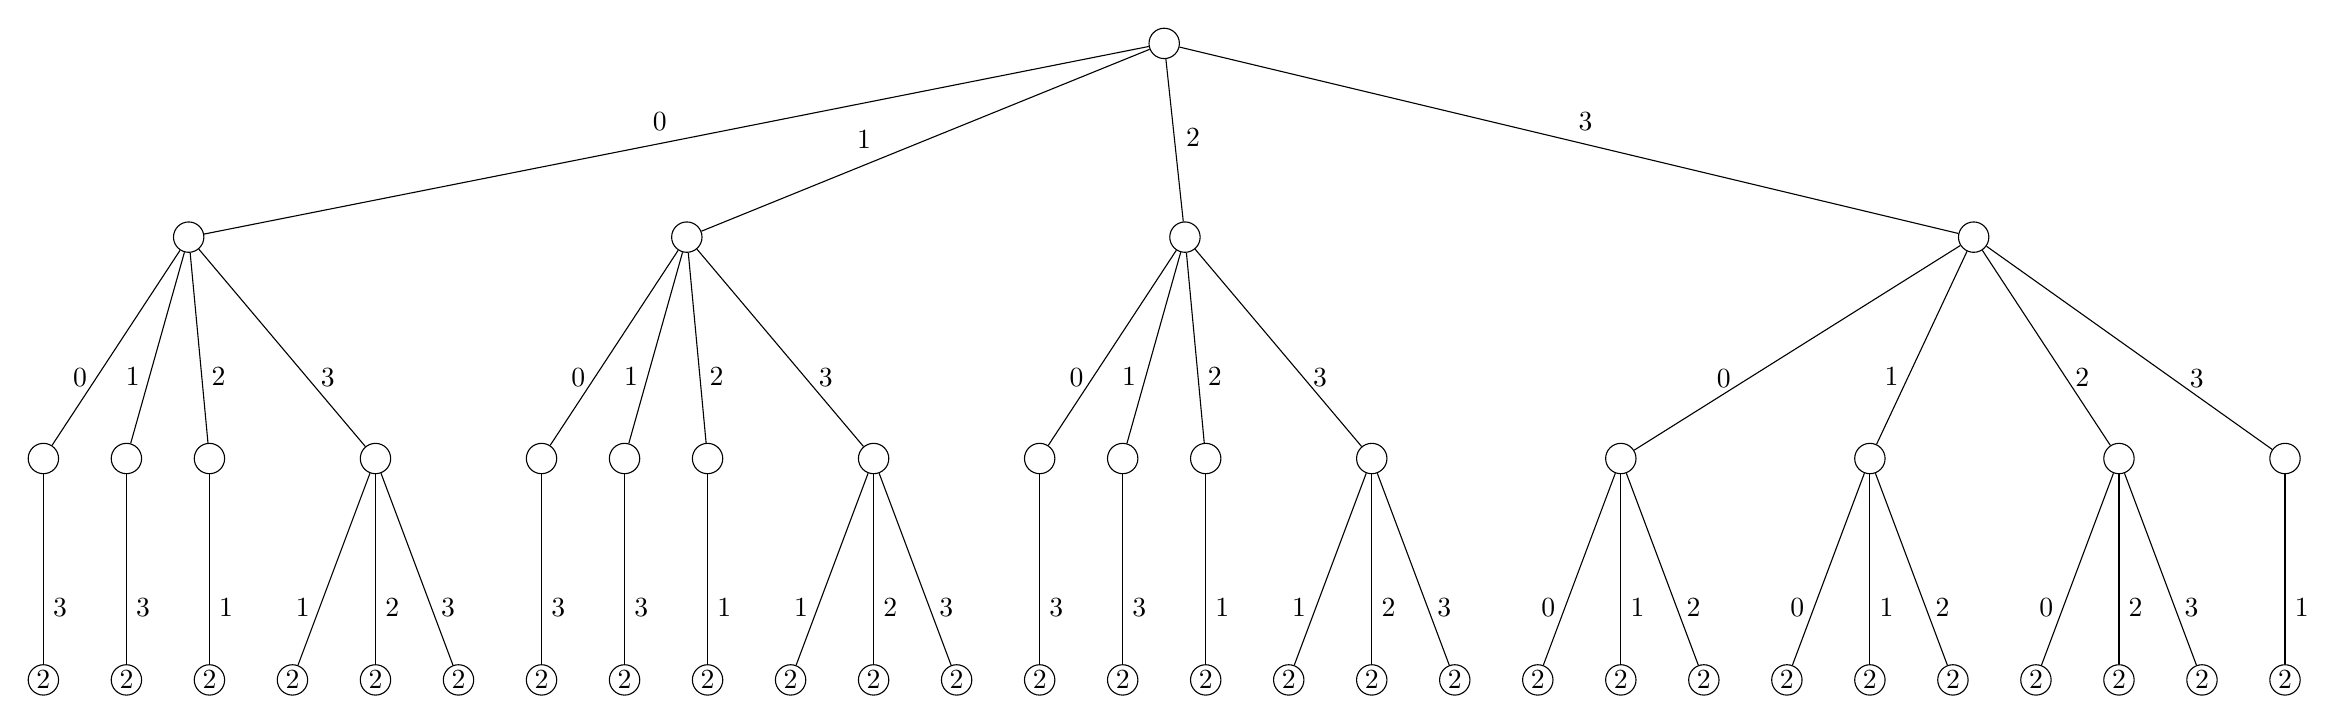
\begin{tikzpicture}[grow=down, edge from parent/.style={draw, -latex}]
    \label{fig:sea-automaton}

    \node at (0pt, 0pt) (S) [shape=circle,draw,inner sep=1pt] {\phantom{0}};

    \node at (-352.5pt, -70pt) (S0) [shape=circle,draw,inner sep=1pt] {\phantom{0}};
    \node at (-172.5pt, -70pt) (S1) [shape=circle,draw,inner sep=1pt] {\phantom{0}};
    \node at (7.5pt,    -70pt) (S2) [shape=circle,draw,inner sep=1pt] {\phantom{0}};
    \node at (292.5pt,  -70pt) (S3) [shape=circle,draw,inner sep=1pt] {\phantom{0}};

    \node at (-405pt, -150pt) (S00) [shape=circle,draw,inner sep=1pt] {\phantom{0}};
    \node at (-375pt, -150pt) (S01) [shape=circle,draw,inner sep=1pt] {\phantom{0}};
    \node at (-345pt, -150pt) (S02) [shape=circle,draw,inner sep=1pt] {\phantom{0}};
    \node at (-285pt, -150pt) (S03) [shape=circle,draw,inner sep=1pt] {\phantom{0}};

    \node at (-225pt, -150pt) (S10) [shape=circle,draw,inner sep=1pt] {\phantom{0}};
    \node at (-195pt, -150pt) (S11) [shape=circle,draw,inner sep=1pt] {\phantom{0}};
    \node at (-165pt, -150pt) (S12) [shape=circle,draw,inner sep=1pt] {\phantom{0}};
    \node at (-105pt, -150pt) (S13) [shape=circle,draw,inner sep=1pt] {\phantom{0}};

    \node at (-45pt, -150pt) (S20) [shape=circle,draw,inner sep=1pt] {\phantom{0}};
    \node at (-15pt, -150pt) (S21) [shape=circle,draw,inner sep=1pt] {\phantom{0}};
    \node at (15pt,  -150pt) (S22) [shape=circle,draw,inner sep=1pt] {\phantom{0}};
    \node at (75pt,  -150pt) (S23) [shape=circle,draw,inner sep=1pt] {\phantom{0}};

    \node at (165pt, -150pt) (S30) [shape=circle,draw,inner sep=1pt] {\phantom{0}};
    \node at (255pt, -150pt) (S31) [shape=circle,draw,inner sep=1pt] {\phantom{0}};
    \node at (345pt, -150pt) (S32) [shape=circle,draw,inner sep=1pt] {\phantom{0}};
    \node at (405pt, -150pt) (S33) [shape=circle,draw,inner sep=1pt] {\phantom{0}};

    \node at (-405pt, -230pt) (F00_3) [shape=circle,draw,inner sep=1pt] {2};
    \node at (-375pt, -230pt) (F01_3) [shape=circle,draw,inner sep=1pt] {2};
    \node at (-345pt, -230pt) (F02_1) [shape=circle,draw,inner sep=1pt] {2};
    \node at (-315pt, -230pt) (F03_1) [shape=circle,draw,inner sep=1pt] {2};
    \node at (-285pt, -230pt) (F03_2) [shape=circle,draw,inner sep=1pt] {2};
    \node at (-255pt, -230pt) (F03_3) [shape=circle,draw,inner sep=1pt] {2};

    \node at (-225pt, -230pt) (F10_3) [shape=circle,draw,inner sep=1pt] {2};
    \node at (-195pt, -230pt) (F11_3) [shape=circle,draw,inner sep=1pt] {2};
    \node at (-165pt, -230pt) (F12_1) [shape=circle,draw,inner sep=1pt] {2};
    \node at (-135pt, -230pt) (F13_1) [shape=circle,draw,inner sep=1pt] {2};
    \node at (-105pt, -230pt) (F13_2) [shape=circle,draw,inner sep=1pt] {2};
    \node at (-75pt,  -230pt) (F13_3) [shape=circle,draw,inner sep=1pt] {2};

    \node at (-45pt,  -230pt) (F20_3) [shape=circle,draw,inner sep=1pt] {2};
    \node at (-15pt,  -230pt) (F21_3) [shape=circle,draw,inner sep=1pt] {2};
    \node at (15pt,   -230pt) (F22_1) [shape=circle,draw,inner sep=1pt] {2};
    \node at (45pt,   -230pt) (F23_1) [shape=circle,draw,inner sep=1pt] {2};
    \node at (75pt,   -230pt) (F23_2) [shape=circle,draw,inner sep=1pt] {2};
    \node at (105pt,  -230pt) (F23_3) [shape=circle,draw,inner sep=1pt] {2};

    \node at (135pt,  -230pt) (F30_0) [shape=circle,draw,inner sep=1pt] {2};
    \node at (165pt,  -230pt) (F30_1) [shape=circle,draw,inner sep=1pt] {2};
    \node at (195pt,  -230pt) (F30_2) [shape=circle,draw,inner sep=1pt] {2};
    \node at (225pt,  -230pt) (F31_0) [shape=circle,draw,inner sep=1pt] {2};
    \node at (255pt,  -230pt) (F31_1) [shape=circle,draw,inner sep=1pt] {2};
    \node at (285pt,  -230pt) (F31_2) [shape=circle,draw,inner sep=1pt] {2};
    \node at (315pt,  -230pt) (F32_0) [shape=circle,draw,inner sep=1pt] {2};
    \node at (345pt,  -230pt) (F32_2) [shape=circle,draw,inner sep=1pt] {2};
    \node at (375pt,  -230pt) (F32_3) [shape=circle,draw,inner sep=1pt] {2};
    \node at (405pt,  -230pt) (F33_1) [shape=circle,draw,inner sep=1pt] {2};

    \path[draw] (S) -- (S0) node [midway, above left, font=\normalsize] {0};
    \path[draw] (S) -- (S1) node [pos=0.6, above left, font=\normalsize] {1};
    \path[draw] (S) -- (S2) node [pos=0.6, above right, font=\normalsize] {2};
    \path[draw] (S) -- (S3) node [midway, above right, font=\normalsize] {3};

    \path[draw] (S0) -- (S00) node [pos=0.65, left, font=\normalsize] {0};
    \path[draw] (S0) -- (S01) node [pos=0.65, left, font=\normalsize] {1};
    \path[draw] (S0) -- (S02) node [pos=0.65, right, font=\normalsize] {2};
    \path[draw] (S0) -- (S03) node [pos=0.65, xshift=0.5mm, right, font=\normalsize] {3};

    \path[draw] (S1) -- (S10) node [pos=0.65, left, font=\normalsize] {0};
    \path[draw] (S1) -- (S11) node [pos=0.65, left, font=\normalsize] {1};
    \path[draw] (S1) -- (S12) node [pos=0.65, right, font=\normalsize] {2};
    \path[draw] (S1) -- (S13) node [pos=0.65, xshift=0.5mm, right, font=\normalsize] {3};

    \path[draw] (S2) -- (S20) node [pos=0.65, left, font=\normalsize] {0};
    \path[draw] (S2) -- (S21) node [pos=0.65, left, font=\normalsize] {1};
    \path[draw] (S2) -- (S22) node [pos=0.65, right, font=\normalsize] {2};
    \path[draw] (S2) -- (S23) node [pos=0.65, right] {3};

    \path[draw] (S3) -- (S30) node [pos=0.65, xshift=-1mm, left, font=\normalsize] {0};
    \path[draw] (S3) -- (S31) node [pos=0.65, left, font=\normalsize] {1};
    \path[draw] (S3) -- (S32) node [pos=0.65, right, font=\normalsize] {2};
    \path[draw] (S3) -- (S33) node [pos=0.65, xshift=1mm, right] {3};

    \path[draw] (S00) -- (F00_3) node [pos=0.7, right, font=\normalsize] {3};
    \path[draw] (S01) -- (F01_3) node [pos=0.7, right, font=\normalsize] {3};
    \path[draw] (S02) -- (F02_1) node [pos=0.7, right, font=\normalsize] {1};
    \path[draw] (S03) -- (F03_1) node [pos=0.7, left, font=\normalsize] {1};
    \path[draw] (S03) -- (F03_2) node [pos=0.7, right, font=\normalsize] {2};
    \path[draw] (S03) -- (F03_3) node [pos=0.7, right, font=\normalsize] {3};

    \path[draw] (S10) -- (F10_3) node [pos=0.7, right, font=\normalsize] {3};
    \path[draw] (S11) -- (F11_3) node [pos=0.7, right, font=\normalsize] {3};
    \path[draw] (S12) -- (F12_1) node [pos=0.7, right, font=\normalsize] {1};
    \path[draw] (S13) -- (F13_1) node [pos=0.7, left, font=\normalsize] {1};
    \path[draw] (S13) -- (F13_2) node [pos=0.7, right, font=\normalsize] {2};
    \path[draw] (S13) -- (F13_3) node [pos=0.7, right, font=\normalsize] {3};

    \path[draw] (S20) -- (F20_3) node [pos=0.7, right, font=\normalsize] {3};
    \path[draw] (S21) -- (F21_3) node [pos=0.7, right, font=\normalsize] {3};
    \path[draw] (S22) -- (F22_1) node [pos=0.7, right, font=\normalsize] {1};
    \path[draw] (S23) -- (F23_1) node [pos=0.7, left, font=\normalsize] {1};
    \path[draw] (S23) -- (F23_2) node [pos=0.7, right, font=\normalsize] {2};
    \path[draw] (S23) -- (F23_3) node [pos=0.7, right, font=\normalsize] {3};

    \path[draw] (S30) -- (F30_0) node [pos=0.7, left, font=\normalsize] {0};
    \path[draw] (S30) -- (F30_1) node [pos=0.7, right, font=\normalsize] {1};
    \path[draw] (S30) -- (F30_2) node [pos=0.7, right, font=\normalsize] {2};

    \path[draw] (S31) -- (F31_0) node [pos=0.7, left, font=\normalsize] {0};
    \path[draw] (S31) -- (F31_1) node [pos=0.7, right, font=\normalsize] {1};
    \path[draw] (S31) -- (F31_2) node [pos=0.7, right, font=\normalsize] {2};

    \path[draw] (S32) -- (F32_0) node [pos=0.7, left, font=\normalsize] {0};
    \path[draw] (S32) -- (F32_2) node [pos=0.7, right, font=\normalsize] {2};
    \path[draw] (S32) -- (F32_3) node [pos=0.7, right, font=\normalsize] {3};

    \path[draw] (S33) -- (F33_1) node [pos=0.7, right, font=\normalsize] {1};

\end{tikzpicture}
}
\caption{Unreduced automaton representation of the SEA S-box DDT.}
\end{figure}

Applying the quaternary reduction rules to this structure removes the repetitive blocks. For instance, in the first level of the automaton, the transitions on symbols \texttt{0}, \texttt{1}, and \texttt{2} are grouped together because their corresponding sub-matrices share an identical structure, immediately sparing half the necessary storage. At the terminal level, only a single accept state is required to represent the differential value 2. The final reduced automaton, shown in Figure~\ref{fig:sea-reduced-automaton}, contains only 8 states, a substantial compression compared to the 64 cells of the original matrix. The function table for $f_{D}$ now contains a single entry mapping the string $\texttt{003}$, corresponding to the only accept state, to the value 2.

\begin{figure}[ht]
\centering
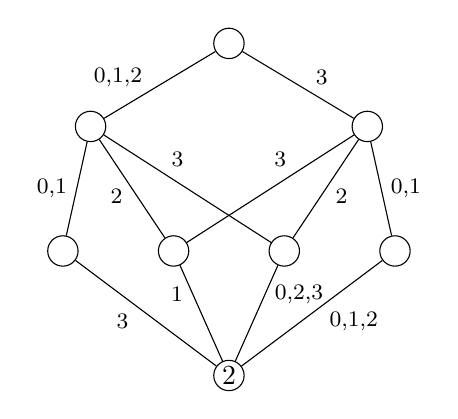
\begin{tikzpicture}[grow=down, level distance=50pt, edge from parent/.style={draw, -latex}]
    \label{fig:sea-reduced-automaton}

    \node (S) [shape=circle,draw,inner sep=1pt] {\phantom{0}};

    \node at (-50pt, -30pt) (S0) [shape=circle,draw,inner sep=1pt] {\phantom{0}};
    \node at (50pt, -30pt) (S3) [shape=circle,draw,inner sep=1pt] {\phantom{0}};
    
    \node at (-60pt, -75pt) (S00) [shape=circle,draw,inner sep=1pt] {\phantom{0}}; % 0002
    \node at (-20pt, -75pt) (S02) [shape=circle,draw,inner sep=1pt] {\phantom{0}}; % 0200
    \node at (20pt, -75pt) (S03) [shape=circle,draw,inner sep=1pt] {\phantom{0}}; % 2022
    \node at (60pt, -75pt) (S30) [shape=circle,draw,inner sep=1pt] {\phantom{0}}; % 2220

    \node at (0pt, -120pt) (F2) [shape=circle,draw,inner sep=1pt] {2};

    \path[draw] (S) -- (S0) node [midway, left, xshift=-1mm, yshift=1mm, font=\footnotesize] {0,1,2};
    \path[draw] (S) -- (S3) node [midway, right, xshift=1mm, yshift=1mm, font=\footnotesize] {3};

    \path[draw] (S0) -- (S00) node [midway, left, font=\footnotesize] {0,1};
    \path[draw] (S0) -- (S02) node [midway, left, yshift=-1mm, font=\footnotesize] {2};
    \path[draw] (S0) -- (S03) node [pos=0.3, right, xshift=1mm, yshift=1mm, font=\footnotesize] {3};
    \path[draw] (S3) -- (S30) node [midway, right, font=\footnotesize] {0,1};
    \path[draw] (S3) -- (S03) node [midway, right, yshift=-1mm, font=\footnotesize] {2};
    \path[draw] (S3) -- (S02) node [pos=0.3, left, xshift=-1mm, yshift=1mm, font=\footnotesize] {3};
    

    \path[draw] (S00) -- (F2) node [midway, left, xshift=-1mm, yshift=-1mm, font=\footnotesize] {3};
    \path[draw] (S02) -- (F2) node [pos=0.3, left, font=\footnotesize] {1};
    \path[draw] (S03) -- (F2) node [pos=0.3, right, font=\footnotesize] {0,2,3};
    \path[draw] (S30) -- (F2) node [midway, right, xshift=1mm, yshift=-1mm, font=\footnotesize] {0,1,2};

\end{tikzpicture}
\caption{SEA reduced automaton.}
\end{figure}



\section{Results}
\label{sec:results}

We evaluated the proposed representation using S-boxes of different sizes from widely used ciphers and vectorial Boolean functions, ranging from $n = 3$ to $n = 8$. For each, we measured the size of the resulting automata compared to the raw table.

\begin{table}
\caption{Comparison between the number of cells in the standard DDT and the number of states and transitions in the proposed automaton representation.}
    \label{tab:compression_results}

    \centering
    \setlength{\tabcolsep}{6pt}

    \begin{tabular}{lrrrr}
        \hline
        
        \textbf{Cipher} & $n$ & \textbf{Cells} & \textbf{States} & \textbf{Transitions} \\
        
        \hline

        SEA & 3 & 64 & 8 & 12 \\
        SKINNY-64 & 4 & 256 & 36 & 63 \\
        PRESENT & 4 & 256 & 38 & 89 \\
        PRINCE & 4 & 256 & 47 & 106 \\
        DryGASCON128 & 5 & 1,024 & 96 & 225 \\
        Ascon & 5 & 1,024 & 106 & 256 \\
        Dillon & 6 & 4,096 & 356 & 1,188 \\
        WAGE & 7 & 16,384 & 1,516 & 4,965 \\
        SKINNY-128 & 8 & 65,536 & 922 & 2,334 \\
        Camellia & 8 & 65,536 & 5,388 & 19,096 \\
        AES & 8 & 65,536 & 5,393 & 19,106 \\
        CLEFIA ($S_{0}$) & 8 & 65,536 & 5,631 & 19,203 \\
        Skipjack & 8 & 65,536 & 5,652 & 19,359 \\
        Safer & 8 & 65,536 & 5,655 & 18,535 \\
        DryGASCON256 & 9 & 262,144 & 4,739 & 14,049 \\
        
        \hline
    \end{tabular}
\end{table}


Table~\ref{tab:compression_results} compares the number of cells in the DDT with the number of states and transitions of our automaton for each S-box. The compression capability is noticeable even for small S-boxes ($n \leq 4$), where the number of states is approximately 5.4 to 8 times smaller than the number of cells. As the size of the S-box increase, this rate also tends to increase, ranging from 9.7 up to 12.2. There are also some S-boxes, like SKINNY-128 and DryGASCON256, in which the rates are much higher (71 and 55.3, respectively), which is a clear signal of their structural regularities. This substantial reduction in the number of required elements suggests a corresponding decrease in practical storage requirements, which we analyze next.

To assess the practical efficiency of this representation, we define a memory layout for the automaton. We assume a contiguous array structure where each state is represented by four fields, corresponding to the transitions for each symbol in the alphabet. Each field stores the index of the next state, with the index 0 reserved to represent the dead state. Moreover, we utilize the bytes allocated to accepting states to store the differential value directly, as these have no outgoing transitions. The size of the transition indices depends on the total number of states $|S|$. If $|S| \leq 255$, 1-byte indices are sufficient, resulting in a state size of 4 bytes. If $255 < |S| \leq 65,535$, we require 2-byte indices, increasing the state size to 8 bytes. This compact layout allows us to calculate the precise memory footprint for each S-box.

\begin{table}
    \centering
    \caption{Memory usage comparison. The ``Autom.'' column details the size of our proposed structure using the layout described in \ref{sec:automaton}. ``DDT Pract.'' assumes a standard 1-byte per cell implementation. ``DDT Theor'' represents the theoretical minimum storage assuming optimal bit-packing for even values between 0 and $\delta$.}
    \label{tab:memory_usage}
    \setlength{\tabcolsep}{6pt}

    \begin{tabular}{lrrrrrr}
        \toprule
        
        \textbf{Cipher} & $n$ & $\delta$ & $|S|$ & \textbf{Autom.} & \textbf{DDT} & \textbf{DDT} \\
         
         & & & & & \textbf{(Pract.)} & \textbf{(Theor.)} \\
        
        \midrule
        
        SEA              & 3 &   2 &     9 &     36 B &  64 B &      8 B \\
        SKINNY-64        & 4 &   4 &    37 &    148 B & 256 B &    64 B \\
        PRESENT          & 4 &   4 &    39 &    156 B & 256 B &    64 B \\
        PRINCE           & 4 &   4 &    48 &    192 B & 256 B &    64 B \\
        DryGASCON128     & 5 &   8 &    97 &    388 B &  1 KB &    384 B \\
        Ascon            & 5 &   8 &   107 &    428 B &  1 KB &    384 B \\
        Dillon           & 6 &   2 &   357 &  2,856 B &  4 KB &    512 B \\
        WAGE             & 7 &   8 & 1,518 & 12,144 B &  16 KB &    6 KB \\
        SKINNY-128       & 8 &  64 &   927 &  7,416 B &  64 KB &   48 KB \\
        Camellia         & 8 &   4 & 5,389 & 43,112 B &  64 KB &   16 KB \\
        AES              & 8 &   4 & 5,394 & 43,152 B &  64 KB &   16 KB \\
        CLEFIA ($S_{0}$) & 8 &  10 & 5,635 & 45,080 B &  64 KB &   24 KB \\
        Skipjack         & 8 &  12 & 5,653 & 45,224 B &  64 KB &   24 KB \\
        Safer            & 8 & 128 & 5,657 & 45,256 B &  64 KB &   56 KB \\
        DryGASCON256     & 9 & 130 & 4,744 & 37,952 B & 256 KB & 224 KB \\

        \bottomrule
    \end{tabular}
\end{table}


Table~\ref{tab:memory_usage} details the memory usage, comparing our proposed representation, in column ``Autom.'', against a standard practical DDT implementation, in column ``DDT Pract.'', that allocates 1 byte per cell. To provide a lower bound for comparison, we also include the ``DDT Theor.'' column, which represents the theoretical minimum storage required. This model assumes an optimal bit-packing strategy that stores only the bits necessary to represent distinct even values between $0$ and $\delta$. Specifically, the total size is calculated as $2^{2n} \times \lceil \log_{2}(\delta / 2 + 1) \rceil$ bits. For example, APN functions like those by Dillon et al. would theoretically require only 1 bit per cell, while the Safer S-box requires 7 bits.

The results in Table~\ref{tab:memory_usage} confirm that the automaton's structural compression translates into memory savings. For SKINNY-128 ($n=8$), the standard DDT requires 64 KB, while our automaton requires only around 7.4 KB. Even for S-boxes with higher differential uniformity like Safer, the automaton representation remains more compact than the practical byte-aligned DDT.
\section{Applications}
\label{sec:applications}

\subsection{Calculating differential properties}

The proposed representation of the difference distribution table allows for the efficient computation of cryptographic metrics without the need to exhaustively generate the standard tabular format. In the following, we demonstrate how each of the differential properties introduced previously can be calculated using this data structure.

To calculate the differential uniformity, it is sufficient to inspect the values stored at the terminal nodes of the data structure. Let $T$ be the set of all terminal nodes. Since the differential uniformity is the maximum frequency of any non-trivial differential, it corresponds directly to the maximum integer value among these nodes. Finding this maximum requires a simple traversal, which takes $\mathcal{O}(|T|)$ time. Since the number of terminal nodes is at most $\Delta_{F}$, the cost is negligible compared to the size of the original DDT.

To compute the differential spectrum, we traverse the automaton starting from the root using a standard search algorithm, such as depth-first search. During the traversal, we track the multiplicity of the current path by multiplying the number of valid transition symbols along each traversed edge. When a terminal node storing a value $i$ is reached, the accumulated path weight is added to the corresponding counter $\omega_i$. This approach requires $\mathcal{O}(D)$ memory, where $D$ is the depth of the automaton and is bounded by the input size $n$. The time complexity is $\mathcal{O}(P)$, where $P$ is the total number of distinct valid paths in the reduced structure.

Impossible differentials, which correspond to zero-entries in the difference distribution table, can also be efficiently extracted from the data structure. To determine if a differential $(a, b)$ is impossible, it suffices to evaluate its encoding, where symbols are formed by the respective bits of $a$ and $b$. That is, if $a = 101$ and $b = 011$, the encoding of the differential $(a, b)$ is the symbol sequence $213$, since the bit pairs from most to least significant are $(1,0)$, $(0,1)$, and $(1,1)$. Since the automaton only accepts non-zero entries, the differential is impossible if and only if its encoding is not in $L(DDT)$. However, for verifying a single specific differential, this traversal is not computationally advantageous compared to a standard DDT. While a direct table lookup operates in $\mathcal{O}(1)$ time, evaluating through the automaton requires $\mathcal{O}(D)$ operations. While this overhead makes the automaton less efficient than a DDT for single-point evaluations, the $\mathcal{O}(D)$ cost remains bounded by the input size $n$ and may not represent a concern. Next, we present methods for performing more complex queries on the automaton, enabling the simultaneous extraction of multiple impossible differentials and other properties.

\subsection{Complex Queries via Automata Operations}
\label{sec:queries}

The transformation of the DDT into a finite automaton establishes a formal
language containing the data in the table. By treating the set of valid
differentials as a language, complex cryptanalytic queries can be
formulated as regular expressions and resolved as operations on this
language. This transforms the ad-hoc process of searching for specific
differential properties into an automated, language-theoretic problem.
Formally, the query process follows these steps:
\begin{enumerate}
    \item The query is formulated as a regular expression $R$ over the
          alphabet $\Sigma$.
    \item The regular expression $R$ is compiled into a finite automaton
          $Q$.
    \item The intersection of $D$ and $Q$ is computed using methods such
          as topological dynamic programming with bit-parallelism or lazy
          depth-first search.
    \item The resulting intersection language is then enumerated, yielding
          the set of DDT entries that satisfy the properties specified by
          the regular expression $R$.
\end{enumerate}

This formal language approach provides a highly flexible mechanism. Rather
than developing custom algorithms for specific search criteria, an analyst
simply constructs the appropriate regular expression. Moreover, because
the class of regular languages is closed under union, intersection, and
complement, complex queries can be assembled compositionally from simpler
ones without leaving the framework. The same query automata can be combined
with the complement of $D$ to reason about impossible differentials, with a
value-restricted sub-automaton of $D$ to filter by probability, or with each
other to express conjunctive constraints.

Throughout the rest of this section, we write the input difference as
$a = a_{n-1}\cdots a_0$ and the output difference as $b = b_{n-1}\cdots
b_0$. Following the encoding of Section~3, each symbol of the word
representing $(a,b)$ is built from a pair of bits $(a_i, b_i)$, so the
four symbols partition naturally into two pairs: symbols
$\{\texttt{0},\texttt{2}\}$ correspond to $a_i = 0$ (input bit
inactive) and symbols $\{\texttt{1},\texttt{3}\}$ to $a_i = 1$ (input
bit active), while symbols $\{\texttt{0},\texttt{1}\}$ correspond to
$b_i = 0$ (output bit inactive) and symbols $\{\texttt{2},\texttt{3}\}$
to $b_i = 1$ (output bit active). For brevity, we display regular
expressions in typewriter font and adopt the usual convention that the
dot \texttt{.} matches any symbol of $\Sigma$, that is, \texttt{.}
$\equiv$ \texttt{(0|1|2|3)}. To illustrate the practical utility of
this method, the following examples demonstrate how common queries can
be formulated for a DDT of size $2^n$.

\begin{itemize}
    \item Fixed input differences: To identify all possible output
          differences for a specific $n$-bit input difference
          $a = \texttt{0101}$, the regular expression is formulated as
          \[
              R = \texttt{(0|2)(1|3)(0|2)(1|3)}.
          \]
          This query replaces the conventional $O(2^n)$ row scan required
          in a standard DDT. Furthermore, it can be reused for other
          values of $a$ by simply changing the transition symbols in the
          query automaton.

    \item Partial and truncated differentials: To evaluate a truncated
          differential where only the two most significant input bits are
          fixed to $\texttt{10}$, the regular expression is formulated as
          \[
              R = \texttt{(1|3)(0|2)..}
          \]
          More generally, any pattern in $\{0,1,*\}^{n}$ on input bits and
          $\{0,1,*\}^{n}$ on output bits maps to a length-$n$ regular
          expression with at most four alternatives per position, so that
          any truncated query of arbitrary mask shape compiles into an
          automaton of $O(n)$ states. The special case in which each
          position is constrained only to be active or inactive (rather
          than fixed to a specific bit value) recovers the activity
          patterns that underlie the MILP- and SAT-based active-S-box
          counts of Mouha et al.~\cite{MouhaEtAl2012} and the differential and linear
          bounds of ciphers such as SKINNY~\cite{BeierleEtAl2016}.

    \item Impossible differentials: Impossible differentials are precisely
          the words rejected by $D$. Rather than testing individual pairs
          $(a,b)$, the framework exposes the entire impossible language
          as the complement
          \[
              L(I) = \overline{L(D)} \cap \Sigma^{n},
          \]
          which is recognized by the complement automaton $\overline{D}$.
          For instance, to enumerate all impossible differentials of a
          $4$-bit S-box whose input has only the least significant bit
          active ($a = \texttt{0001}$, $b$ unconstrained), the regular
          expression is
          \[
              R = \texttt{(0|2)(0|2)(0|2)(1|3)},
          \]
          and the impossible cells of that row are read from
          $\overline{L(D)} \cap L(R)$. This is the elementary
          building block of impossible-differential cryptanalysis as
          first applied to Skipjack~\cite{BihamEtAl1999} and DEAL~\cite{Knudsen1998}, where one
          routinely needs the full set of zero-entries that respect a
          given activity pattern.

    \item Extremal-probability differentials: Because the reduced
          automaton stores the differential multiplicity directly on
          each accepting state, filtering by probability does not
          require any path enumeration: it is a one-pass scan of the
          state set. Let $D_{\geq \tau}$ denote the sub-automaton
          obtained from $D$ by retaining only the accepting states
          whose stored value is at least $\tau$ and pruning unreachable
          states. Then $L(D_{\geq \tau})$ is the set of differentials
          with probability at least $\tau \cdot 2^{-n}$, and the
          differentials achieving the differential uniformity
          $\Delta(F)$ are obtained by setting $\tau = \Delta(F)$. For
          the PRESENT S-box~\cite{BogdanovEtAl2007}, where $n = 4$ and $\Delta = 4$, the
          language $L(D_{\geq 4})$ enumerates the handful of
          high-probability transitions that anchor the best known
          characteristics of the cipher; choosing $\tau = 2$ instead
          returns every non-trivial valid transition that is available
          to a trail. This is exactly the seed information consumed by
          branch-and-bound differential trail searches such as
          Matsui's~\cite{Matsui1995} and its modern MILP and SAT descendants. The
          construction of $D_{\geq \tau}$ visits each accepting state
          at most once, so it runs in $O(|S|)$ time independently of
          the size of the resulting language.

    \item Hamming-weight bounded differentials: Many design strategies and
          search heuristics rely on input and output differences of low
          Hamming weight, since these often dominate the best multi-round
          trails. The set of words encoding differentials with
          $\mathrm{wt}(a) + \mathrm{wt}(b) \leq w$ is recognized by a
          counter automaton with $O(n\,w)$ states: at each position, the
          automaton increments its weight counter by $0$, $1$, or $2$
          depending on whether the symbol is $\texttt{0}$, in
          $\{\texttt{1},\texttt{2}\}$, or $\texttt{3}$.
          For example, restricting to single-bit input and output
          ($\mathrm{wt}(a) = \mathrm{wt}(b) = 1$) is recognized by the
          regular expression
          \[
              R = \texttt{0}^{*}\texttt{2}\,\texttt{0}^{*}\texttt{1}\,\texttt{0}^{*}\;|\;
                  \texttt{0}^{*}\texttt{1}\,\texttt{0}^{*}\texttt{2}\,\texttt{0}^{*}\;|\;
                  \texttt{0}^{*}\texttt{3}\,\texttt{0}^{*},
          \]
          and its intersection with $D$ enumerates the differentials
          targeted by single-bit and bit-flip distinguishers.
          Intersecting more general counter automata with $D$ supports
          the wide-trail strategy of Daemen and Rijmen~\cite{DaemenRijmen2002}, in which
          the designer must verify that no low-weight differential of a
          chosen S-box falls below the targeted probability threshold.

    \item Linearly constrained differentials: Linear relations on the
          bits of $(a,b)$ arise naturally when an S-box is embedded in
          a larger primitive. In a multi-round setting, the linear
          layer that follows a round of S-boxes constrains how the
          output differences of one round map to the input differences
          of the next, which translates, after fixing the surrounding
          differences, into a linear constraint on each S-box's local
          $(a,b)$. The simplest such constraint is the diagonal
          relation $a = b$, which is recognized by the regular
          expression
          \[
              R = \texttt{(0|3)}^{n},
          \]
          since symbols $\texttt{0}$ and $\texttt{3}$ are exactly those
          with $a_i = b_i$.
          More generally, any $\mathbb{F}_{2}$-linear relation on the
          bits of $(a,b)$ is recognized by a deterministic automaton
          whose states track the running parities of the relation, with
          at most $2^{r}$ states for $r$ independent linear constraints.
          Intersecting such an automaton with $D$ extracts exactly the
          DDT entries that are compatible with the linear context, a
          search that traditionally requires either bespoke filters or
          auxiliary MILP or SAT formulations.

    \item Composite queries: Because regular languages are closed under
          boolean operations, the previous queries can be combined freely.
          A concrete example is the search for high-probability
          low-weight differentials, formulated as the intersection
          \[
              L(D_{\geq \Delta(F)/2}) \cap L(\mathrm{wt} \leq 2),
          \]
          which is precisely the kind of seed used by trail-search
          heuristics for ciphers such as PRESENT~\cite{BogdanovEtAl2007} and SKINNY~\cite{BeierleEtAl2016},
          where only differentials that are both probable enough to
          contribute and sparse enough to survive the diffusion layer
          need to be retained. Other useful combinations include the
          intersection of $\overline{D}$ with a truncated query, which
          enumerates activity patterns guaranteed to vanish across one
          S-box layer, and the intersection of a linear-constraint
          automaton with a truncated query, which filters
          the differentials that survive a linear layer while
          respecting a required activity pattern. Each compound query
          is built by a single automata product and inherits the same
          enumeration and counting primitives as the elementary ones.

    \item Comparing two DDTs: The framework also supports queries that
          span two S-boxes. Given automata $D_F$ and $D_G$ for the DDTs
          of $F$ and $G$, the language $L(D_F) \setminus L(D_G)$
          collects the differentials that are possible for $F$ but
          impossible for $G$, and $L(D_F) \cap L(D_G)$ collects those
          shared by both. Such operations are useful for comparing
          candidate S-boxes during the design of a cipher: members of
          the same affine-equivalence class share the same DDT up to a
          relabelling of inputs and outputs, so $L(D_F) \setminus
          L(D_G)$ provides a direct certificate of inequivalence,
          while comparing two candidates from different equivalence
          classes (a situation that arises, for example, in the S-box
          selection of lightweight ciphers such as PRINCE~\cite{BorghoffEtAl2012} and
          Midori~\cite{BanikEtAl2015}) isolates the differentials that distinguish
          their behaviour under a fixed differential property of
          interest.
\end{itemize}

For all of the queries above, the running time is dominated by the size
of the intersection language, which is bounded by $|D| \cdot |Q|$ in the
worst case, but is usually much smaller in practice because most query
automata are sparse and length-deterministic. The intersection is not
materialized explicitly; following the workflow at the start of this
section, it is computed by a joint traversal of $D$ and $Q$ (lazy
depth-first search) or by a topological dynamic program with
bit-parallelism over the two automata. Critically, no query above visits
the dense $2^{n} \times 2^{n}$ matrix, even implicitly: the only objects
touched are the already-compressed automaton $D$ and the small query
automaton $Q$, so the asymptotic memory savings of Section~4 carry over
to query time. This makes the representation particularly attractive
for cryptanalytic workflows that revisit the DDT many times under
varying constraints.

\section{Conclusion}
\label{sec:conclusion}

This paper discussed an automaton-theoretic representation for the
differential distribution tables. We outlined the memory constraints
inherent in differential cryptanalysis, presented a method that reframes
DDTs as formal languages, and proposed representing them using finite
automata to capture structural regularities. We validated this
representation by evaluating its memory usage across various S-boxes,
confirming that the structural compression translates into concrete storage
advantages over standard matrix implementations.

Representing a DDT as a dense matrix provides straightforward access but
suffers from exponential growth, becoming prohibitive for storage as S-box
sizes increase. These constraints force researchers to limit the scope of
their analysis, either by restricting the size of the primitives analyzed
or by relying on simplifications and heuristics. By exploiting the
redundancies present in typical S-boxes, we demonstrated that this tabular
structure can be substantially compressed without any loss of data, opening
the possibility of extending the practical boundaries of analysis.

Beyond the storage gains, the central observation of this work is that the
language-theoretic view does more than reduce memory. Once the DDT is
expressed as a regular language, the cryptanalytic searches that an
analyst performs over the table become operations on automata, and the
wide range of properties that can be phrased as regular conditions over
the quadrant encoding of $(a,b)$ are all recovered through a single
joint traversal of the DDT automaton and a small query automaton. We
described several such queries, covering
fixed-input and truncated differentials, impossible differentials,
extremal-probability entries, low-weight transitions, linearly constrained
pairs, composite queries built by boolean closure, and
cross-DDT comparisons. Each of these tasks, historically implemented by a
bespoke scan of the dense table, becomes a short regular expression in the
proposed framework and inherits the compactness of the underlying
automaton.

Several directions naturally extend the present work. The query catalogue
can be enriched with non-regular but context-free constraints, such as
bounded-difference balances across multiple rounds, by replacing the
query automaton with a pushdown automaton and adapting the joint
traversal accordingly.
The same automaton can also serve as a generator of linear inequalities
for MILP-based trail search, providing an alternative route to the
modeling of S-box behavior; a careful study of the trade-off between
automaton size and the number of generated inequalities is left to future
work. Finally, the size of the reduced automaton itself appears to capture
an intrinsic notion of structural regularity of an S-box, and quantifying
the deviation between an actual DDT and its random or theoretically
optimal counterparts via this size-based metric is a natural analytical
follow-up.


% -----------------------------

\newpage

%
% ---- Bibliography ----
%
% BibTeX users should specify bibliography style 'splncs04'.
% References will then be sorted and formatted in the correct style.
%
\bibliographystyle{splncs04}
\bibliography{bibligraphy}

\end{document}
